\section{Examples}
\label{sect:gmas:examples}

We now discuss various instantiations of argument schemes and the result of answering critical questions in more detail. For each example we provide transcript excerpts, a visualization of the arguments, and the corresponding goal model elements. We provide a legend for our visualization notation in Figure~\ref{fig:legend}.

\begin{figure}[ht!]
\centering
\begin{tikzpicture}
        \node (att1) [argNodeIN] at (-5,0) {$A_1$};
        \node (att2) [argNodeOUT] at (-2,0) {$A_2$};
        \node (attDescription) [draw=none, align=center] at (0.5,0) {Argument $A_1$ (accepted)\\ attacks argument $A_2$\\ (rejected)};
        \node[traceNodeGREEN] (trace1a) at (-5,-1.5) {};
        \node[traceNodeGREEN] (trace1b) at (-2,-1.5) {};
        \node (traceDescription) [draw=none,align=center] at (0.5,-1.5) {Traceability link from\\ accepted argument to\\ enabled GRL element};
        \node[traceNodeRED] (trace2a) at (-5,-3) {};
        \node[traceNodeRED] (trace2b) at (-2,-3) {};
        \node (traceDescription) [draw=none,align=center] at (0.5,-3) {Traceability link from\\ rejected argument to\\ disabled GRL element};
        \node (cq1) [argNodeIN] at (-5,-4.5) {$A_1$};
        \node (cq2) [argNodeIN] at (-2,-4.5) {$A_2$};
        \node (cqDescription) [draw=none,align=center] at (0.5,-4.5) {Argument $A_2$ is the result of\\ answering critical question\\ $CQ$ of argument $A_1$};
         \path
    (att1) edge [attackLink] (att2)
    (cq1) edge [CQLink] node [above,draw=none] {CQ} (cq2)
    (trace1a) edge[traceLinkGREEN] (trace1b)
    (trace2a) edge[traceLinkRED] (trace2b);
\end{tikzpicture}
\caption{Legend of the various elements and relationships we use for the examples in this article.}
\label{fig:legend}
\end{figure}


\subsubsection{Example 1: Disable task \texttt{Traffic light}}

The transcript excerpt of this example is shown in Table~\ref{table:transcripts:traffic-light} in the appendix and comes from transcript $t_1$. In this example, participants are summing up functionality of the traffic simulator, which are tasks that the student can perform in the simulator. All these task can be formalized and are instantiations of argument scheme AS2: ``Actor \emph{Student} has tasks $T$'', where $T\in\{$Save map, Open map, Add intersection, Remove intersection, Add road, Add traffic light$\}$''. 

Once all these tasks are summed up, participant \texttt{P1} notes that the problem description states that all intersections in the traffic simulator have traffic lights, so the task \texttt{Add traffic light} is not useful. We formalized this using the critical question CQ12: ``Is task \texttt{Add traffic light} useful/relevant?''.

We visualize some of the argument schemes, critical questions, and traceability links with the GRL model in Figure~\ref{fig:examples:traffic-light}. On the left side of the image, we see three of the instantiated argument schemes AS2. The bottom one, ``Actor \texttt{Student} has task \texttt{Add traffic light}'', is attacked by another argument generated from applying critical question CQ12: ``\texttt{Add traffic light} is useless (\emph{All intersections have traffic lights}). As a result, the corresponding GRL task is disabled. The other two tasks are enabled and have green traceability links.

\begin{figure}[ht!]
\centering
        \begin{tikzpicture}
        \node (a0) [argNodeIN] at (-2,0) {
        	\argtext{AS2}{Actor \emph{Student} has task \emph{Save map}}
        };
        \node (a1) [argNodeIN] at (-2,-2) {
        	\argtext{AS2}{Actor \emph{Student} has task \emph{Add road}}
        };
        \node (a2) [argNodeOUT] at (-2,-4) {
        	\argtext{AS2}{Actor \emph{Student} has task \emph{Add traffic light}}
        };
        \node (a3) [argNodeIN] at (-2,-6){
        	\argtext{}{\emph{Add traffic light} is useless (\emph{All intersections have traffic lights})}
        };
        \node[grl] (task1) at (2.3,0) { 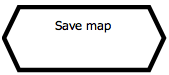
\includegraphics[scale=0.5]{img/task_save_map} };
        \node[grl] (task2) at (2.3,-2) { 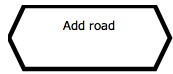
\includegraphics[scale=0.5]{img/task_add_road} };
        \node[grl, disabled] (task3) at (2.3,-4) { 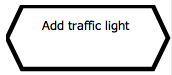
\includegraphics[scale=0.5]{img/task_add_traffic_light} };
        \node[traceNodeGREEN] (trace1a) at (-.4,-.3) {};
        \node[traceNodeGREEN] (trace1b) at (2.2,-.3) {};
        \node[traceNodeGREEN] (trace2a) at (-.4,-2.3) {};
        \node[traceNodeGREEN] (trace2b) at (2.2,-2.3) {};
        \node[traceNodeRED] (trace3a) at (-.4,-4.3) {};
        \node[traceNodeRED] (trace3b) at (2.2,-4.3) {};
         \path
    (a3) edge [attackLink] (a2)
    (a2) edge [CQLink, bend right=50] node [left,draw=none] {CQ12} (a3)
    (trace1a) edge[traceLinkGREEN] (trace1b)
    (trace2a) edge[traceLinkGREEN] (trace2b)
    (trace3a) edge[traceLinkRED] (trace3b);
\end{tikzpicture}
\caption{Argument schemes and critical questions (left), GRL model (right), and traceability link (dotted lines) for the traffic light example.}
\label{fig:examples:traffic-light}
\end{figure}


\subsubsection{Example 2: Clarify task \texttt{Road pattern}}

The transcript excerpt of the second example is shown in Table~\ref{table:transcript:task-clarification} in Appendix~\ref{sect:transcripts:excerpts} and comes from transcript $t_3$. It consists of a number of clarification steps, resulting in the task \texttt{Choose a road pattern}. 

\begin{figure}[ht!]
\centering
        \begin{tikzpicture}[->]
        \node (a0) [argNodeOUT] at (-2,0) {
        	\argtext{AS2}{Actor \emph{Student} has task \emph{Create road}}
        };
        \node (a1) [argNodeOUT] at (-2,-2) {
        	\argtext{AS2}{Actor \emph{Student} has task \emph{Choose a pattern}}
        };
        \node (a2) [argNodeOUT] at (-2,-4.2) {
        	\argtext{AS2}{Actor \emph{Student} has task \emph{Choose a pattern preference}}
        };
        \node (a3) [argNodeIN] at (-2,-6.7) {
        	\argtext{AS2}{Actor \emph{Student} has task \emph{Choose a road pattern}}
        };
        \node[grl] (actor) at (2.3,-4) { 
        	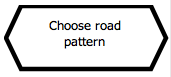
\includegraphics[scale=0.5]{img/task_choose_road_pattern} 
        };
        \node[traceNodeGREEN] (trace1) at (-.5,-7.1) {};
        \node[traceNodeGREEN] (trace2) at (2.2,-4.4) {};

\begin{pgfonlayer}{background}
         \path
    (a1) edge[attackLink] (a0)
    (a2) edge[attackLink] (a1)
    (a2) edge[attackLink, bend right=20] (a0)
    (a3) edge[attackLink] (a2)
    (a3) edge[attackLink, bend right=20] (a1)
    (a3) edge[attackLink, bend right=40] (a0);
\end{pgfonlayer}

	\path
	(a0) edge [CQLink, bend right=50] node [left,draw=none] {CQ12a} (a1)
    (a1) edge [CQLink, bend right=50] node [left,draw=none] {CQ12a} (a2)
    (a2) edge [CQLink, bend right=50] node [left,draw=none] {CQ12a} (a3)
    (trace1) edge[traceLinkGREEN] (trace2);
\end{tikzpicture}
\caption{Argument schemes and critical questions (left), GRL model (right), and traceability link (dotted line) of the road pattern example.}
\label{fig:examples:clarification}
\end{figure}

The formalized argument schemes and critical questions are shown in Figure~\ref{fig:examples:clarification}. The discussion starts with the first instantiation of argument scheme AS2: ``Actor \texttt{Student} has task \texttt{Create road}''. This argument is then challenged with critical question CQ12: ``Is the task \texttt{Create road} clear?''. Answering this question results in a new instantiation of argument scheme AS2: ``Actor \texttt{Student} has task \texttt{Choose a pattern}''. This process is repeated two more times, resulting in the final argument ``Actor \texttt{Student} has task \texttt{Choose a road pattern}''. This final argument is unattacked and has a corresponding intentional element (right image). 

What is clearly shown in this example is that a clarifying argument attacks all arguments previously used to describe the element. For instance, the final argument on the bottom of Figure~\ref{fig:examples:clarification} attacks all three other arguments for a name of the element. If this was not the case, then it may occur that a previous argument is \emph{reinstatiated}, meaning that it becomes accepted again because the argument attacking it is itself attacked. Suppose for instance the bottom argument ``Actor \texttt{Student} has task \texttt{Choose a pattern preference}'' did not attack the second argument: ``Action \texttt{Student} has task \texttt{Choose a pattern}''. In that case, this argument would be reinstated, because its only attacker ``Actor \texttt{Student} has task \texttt{Choose a pattern preference}'' is itself defeated by the bottom argument.

\subsubsection{Example 3: Decompose goal \texttt{Simulate}}

The transcript excerpt of this example is shown in Table~\ref{table:transcript:decomposition} in the appendix and comes from transcript $t_3$. It consists of a discussion about the type of decomposition relationship for the goal \texttt{Simulate}.

\begin{figure}[ht!]
\centering
        \begin{tikzpicture}[->]
        \node (a0) [argNodeIN] at (-2,0) {
        	\argtext{AS3}{Actor \emph{System} has goal \emph{Simulate}}
        };
        \node (a1) [argNodeIN] at (-2,-1.5) {
        	\argtext{AS2}{Actor \emph{System} has task \emph{Dynamic simulation}}
        };
        \node (a2) [argNodeIN] at (-2,-3) {
        	\argtext{AS2}{Actor \emph{System} has task \emph{Static simulation}}
        };
        \node (a3) [argNodeOUT] at (-2,-5) {
        	\argtext{AS5}{Goal \emph{Simulate} AND-decomposes into \emph{Static simulation} and \emph{Dynamic simulation}}
        };
        \node (a4) [argNodeIN] at (-2,-7.5) {
        	\argtext{AS5}{Goal \emph{Simulate} OR-decomposes into \emph{Static simulation} and \emph{Dynamic simulation}}
        };
        \node[grl] (actor) at (2.3,-4) { 
        	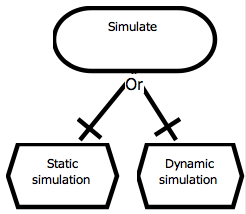
\includegraphics[scale=0.5]{img/simulate_decomposition} 
        };
        \node[traceNodeGREEN] (trace1a) at (-.4,-.3) {};
        \node[traceNodeGREEN] (trace1b) at (2.5,-3.1) {};
        \node[traceNodeGREEN] (trace2a) at (-.4,-1.8) {};
        \node[traceNodeGREEN] (trace2b) at (3.5,-5.6) {};
        \node[traceNodeGREEN] (trace3a) at (-.4,-3.3) {};
        \node[traceNodeGREEN] (trace3b) at (1.3,-5.6) {};
        \node[traceNodeGREEN] (trace4a) at (-.4,-8.2) {};
        \node[traceNodeGREEN] (trace4b) at (2.5,-3.9) {};

\begin{pgfonlayer}{background}
         \path
    (a4) edge[attackLink] (a3);
\end{pgfonlayer}

	\path
	(a3) edge [CQLink, bend right=50] node [left,draw=none] {CQ10b} (a4)
    (trace1a) edge[traceLinkGREEN] (trace1b)
    (trace2a) edge[traceLinkGREEN] (trace2b)
    (trace3a) edge[traceLinkGREEN] (trace3b)
    (trace4a) edge[traceLinkGREEN, bend right] (trace4b);
\end{tikzpicture}
\caption{Argument schemes and critical questions (left), GRL model (right), and traceability link (dotted line) of the goal decomposition example.}
\label{fig:examples:decomposition}
\end{figure}

The visualization of this discussion is shown in Figure~\ref{fig:examples:decomposition}. Each GRL element on the right has a corresponding argument on the left. Moreover, the original argument for an AND-decomposition is attacked by the argument for the OR-decomposition, and the new argument is linked to the decomposition relation in the GRL model.

\subsubsection{Example 4: Reinstate actor \texttt{Development team}}

The transcript excerpt of this example is shown in Table~\ref{table:transcript:irrelevant-actor} in the appendix and comes from transcript $t_3$. It consists of two parts: first participant \texttt{P1} puts forth the suggestion to include actor \texttt{Development team} in the model. This is, then, questioned by participant \texttt{P2}, who argues that the professor will develop the software, so there won't be any development team. However, in the second part, participant \texttt{P2} argue that the development team should be considered, since the professor does not develop the software.

\begin{figure}[ht!]
\centering
        \begin{tikzpicture}
        \node (a0) [argNodeOUT] at (-2,0) {
        	\argtext{AS0}{Development team is relevant}
        } ;
        \node (a1) [argNodeIN] at (-2,-2.5){
        	\argtext{}{Development team is not relevant (\emph{The professor makes the software})}
        };
        \node[grl, disabled] (actor) at (2.3,-1) { 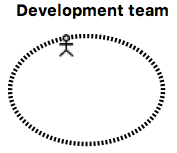
\includegraphics[scale=0.5]{img/actor_development_team} };
        \node[traceNodeRED] (trace1) at (-.5,-.3) {};
        \node[traceNodeRED] (trace2) at (2.2,-0.1) {};

         \path
    (a1) edge[attackLink] (a0)
    (a0) edge [CQLink, bend right=50] node [left,draw=none] {CQ0} (a1)
    (trace1) edge[traceLinkRED] (trace2);
\end{tikzpicture}
\caption{Argument schemes and critical questions (left), GRL model (right), and traceability link (dotted line) of a discussion about the relevance of actor Development team.}
\label{fig:examples:relevant-actor}
\end{figure}

We formalize this using a \emph{generic counterargument}, attacking the critical question. The first part of the discussion is shown in Figure~\ref{fig:examples:relevant-actor}. We formalize the first statement as an instantiation of argument scheme AS0: ``Actor \texttt{development team} is relevant''. This argument is, then, attacked by answering critical question CQ0: ``Is actor \texttt{development team} relevant? with \emph{No}. This results in two arguments, AS0 and CQ0, where CQ0 attacks AS0. This is shown in Figure~\ref{fig:examples:relevant-actor}, left image.

\begin{figure}[ht!]
\centering
        \begin{tikzpicture}
        \node (a0) [argNodeIN] at (-2,0) {
        	\argtext{AS0}{Development team is relevant}
        };
        \node (a1) [argNodeOUT] at (-2,-2.5){
        	\argtext{}{Development team is not relevant (\emph{The professor makes the software})}
        };
        \node (a2) [argNodeIN] at (-2,-5) {
        	\argtext{}{The professor doesn't develop the software}
        } ;
        \node[grl] (actor) at (2.3,-1) { 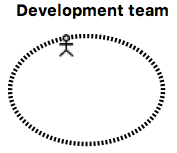
\includegraphics[scale=0.5]{img/actor_development_team} };
        \node[traceNodeGREEN] (trace1) at (-.5,-.3) {};
        \node[traceNodeGREEN] (trace2) at (2.2,-0.1) {};

         \path
    (a1) edge[attackLink] (a0)
    (a2) edge[attackLink] (a1)
    (a0) edge [CQLink, bend right=50] node [left,draw=none] {CQ0} (a1)
    (a1) edge [CQLink, bend right=50] node [left,draw=none] {Att} (a2)
    (trace1) edge[traceLinkGREEN] (trace2);
\end{tikzpicture}
\caption{Argument schemes and critical questions (left), GRL model (right), and traceability link (dotted line) of a discussion about the relevance of actor Development team.}
\label{fig:examples:relevant-actor2}
\end{figure}

Figure~\ref{fig:examples:relevant-actor2} shows the situation after the counter argument has been put forward. The argument ``Actor \texttt{Professor} doesn't develop the software'' now attacks the argument ``\texttt{Development team} is not relevant (\emph{The professor makes the software})'', which in turn attacks the original argument ``\texttt{Development team} is relevant''. As a result, the first argument is reinstated, which causes the actor in the GRL model to be enabled again.